\chapter{Figuren en rechte hoeken}\label{ch:g3:shapes}

Vierkanten, rechthoeken, driehoeken, cirkels: die figuren zijn oude
bekenden. In dit hoofdstuk bekijken we ze met het oog van een meetkundige
--- wat maakt een vierkant precies een vierkant? --- en maak je kennis
met het gereedschap dat beslist: de geodriehoek en zijn \omterm{def:g3:shapes:rightangle}{rechte hoek}.

\section{De rechte hoek}

\begin{definition}[Rechte hoek]\label{def:g3:shapes:rightangle}
Een \emph{rechte hoek}\index{rechte hoek} is de hoek van een blad papier
of van de geodriehoek. Twee lijnen die een rechte hoek maken, staan
\emph{loodrecht} op elkaar. In figuren wordt een rechte hoek aangegeven
met een klein vierkantje in de hoek.
\end{definition}

\begin{method}[Een rechte hoek controleren]\label{met:g3:shapes:check}
\begin{enumerate}
  \item Leg de hoek van de geodriehoek precies op de hoek die je wilt
        testen;
  \item schuif één rand van de geodriehoek langs één zijde van de hoek;
  \item loopt de andere zijde van de hoek precies langs de andere rand,
        dan is de hoek recht --- staat hij wijder of smaller open, dan
        niet.
\end{enumerate}
\end{method}

\begin{omfigure}
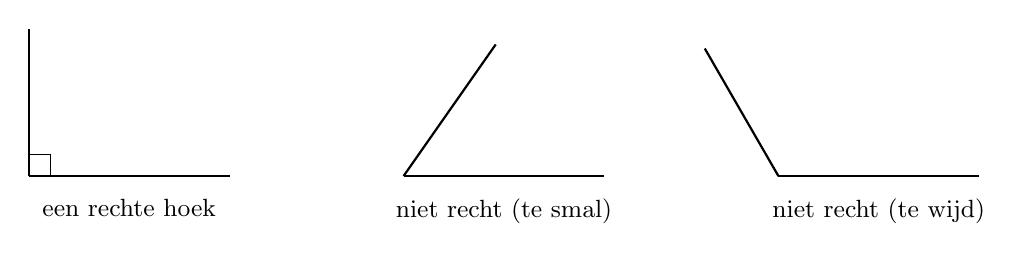
\begin{tikzpicture}[scale=0.85]
  \draw[thick] (0,0) -- (3,0);
  \draw[thick] (0,0) -- (0,2.2);
  \draw[thin] (0.32,0) -- (0.32,0.32) -- (0,0.32);
  \node[below, font=\small] at (1.5,-0.2) {een rechte hoek};
  \begin{scope}[xshift=5.6cm]
  \draw[thick] (0,0) -- (3,0);
  \draw[thick] (0,0) -- (55:2.4);
  \node[below, font=\small] at (1.5,-0.2) {niet recht (te smal)};
  \end{scope}
  \begin{scope}[xshift=11.2cm]
  \draw[thick] (0,0) -- (3,0);
  \draw[thick] (0,0) -- (120:2.2);
  \node[below, font=\small] at (1.5,-0.2) {niet recht (te wijd)};
  \end{scope}
\end{tikzpicture}

{\small Alleen de eerste hoek is recht --- en alleen het vierkantje of de
geodriehoek kan dat garanderen: je ogen laten zich makkelijk bedriegen.}
\end{omfigure}

\section{De figuren en hun regels}

\begin{definition}[Vierkant, rechthoek, driehoek]\label{def:g3:shapes:shapes}
\begin{itemize}
  \item Een \emph{rechthoek}\index{rechthoek} heeft $4$ zijden en $4$
        \omterm{def:g3:shapes:rightangle}{rechte hoeken}; de zijden die tegenover elkaar liggen, zijn even
        lang.
  \item Een \emph{vierkant}\index{vierkant} is een rechthoek waarvan de
        $4$ zijden allemaal even lang zijn.
  \item Een \emph{driehoek}\index{driehoek} heeft $3$ zijden; een
        \emph{rechthoekige driehoek} heeft één \omterm{def:g3:shapes:rightangle}{rechte hoek}.
  \item Een \emph{cirkel}\index{cirkel} teken je met de passer: al zijn
        punten liggen op dezelfde afstand (de \emph{radius}\index{radius})
        van het \emph{middelpunt}.
\end{itemize}
\end{definition}

\begin{omfigure}
\begin{tikzpicture}[scale=0.72]
  % vierkant, met de haakjes voor de rechte hoeken naar binnen getekend
  \draw[thick] (0,0) rectangle (2,2);
  \foreach \x/\y/\dx/\dy in {0/0/1/1, 2/0/-1/1, 0/2/1/-1, 2/2/-1/-1}
    \draw[thin] (\x+0.22*\dx,\y) -- (\x+0.22*\dx,\y+0.22*\dy)
      -- (\x,\y+0.22*\dy);
  \draw (0.93,-0.07) -- (1.07,0.07);
  \draw (0.93,1.93) -- (1.07,2.07);
  \draw (-0.07,0.93) -- (0.07,1.07);
  \draw (1.93,0.93) -- (2.07,1.07);
  \node[below, font=\small] at (1,-0.35) {vierkant};
  % rechthoek
  \begin{scope}[xshift=3.8cm]
  \draw[thick] (0,0) rectangle (3,2);
  \foreach \x/\y/\dx/\dy in {0/0/1/1, 3/0/-1/1, 0/2/1/-1, 3/2/-1/-1}
    \draw[thin] (\x+0.22*\dx,\y) -- (\x+0.22*\dx,\y+0.22*\dy)
      -- (\x,\y+0.22*\dy);
  \node[below, font=\small] at (1.5,-0.35) {rechthoek};
  \end{scope}
  % rechthoekige driehoek
  \begin{scope}[xshift=8.6cm]
  \draw[thick] (0,0) -- (2.6,0) -- (0,2) -- cycle;
  \draw[thin] (0.28,0) -- (0.28,0.28) -- (0,0.28);
  \node[below, font=\small] at (1.3,-0.35) {rechthoekige driehoek};
  \end{scope}
  % cirkel
  \begin{scope}[xshift=13.2cm]
  \draw[thick] (1,1) circle (1.1);
  \fill (1,1) circle (1.5pt);
  \draw[omDef, thick] (1,1) -- ++(45:1.1);
  \node[omDef, font=\small, above right] at (1.72,1.68) {radius};
  \node[below, font=\small] at (1,-0.35) {cirkel};
  \end{scope}
\end{tikzpicture}

{\small De verzameling figuren, met hun tekens: vierkantjes voor \omterm{def:g3:shapes:rightangle}{rechte
hoeken}, streepjes voor gelijke zijden.}
\end{omfigure}

\begin{example}[Waarom die tekens nodig zijn]\label{ex:g3:shapes:marks}
Een figuur die een beetje scheef getekend is, kan op een vierkant
\emph{lijken} zonder er een te zijn. De tekens vertellen de waarheid: $4$
vierkantjes voor de \omterm{def:g3:shapes:rightangle}{rechte hoeken} $+$ $4$ streepjes $=$ een echt
vierkant. Zet de tekens erbij als je zelf tekent; en vertrouw bij het
lezen van een figuur alleen op de tekens en de gegeven maten.
\end{example}

\section{Tekenen op ruitjespapier}

\begin{method}[Constructies op een raster]\label{met:g3:shapes:grid}
Ruitjespapier geeft je \omterm{def:g3:shapes:rightangle}{rechte hoeken} cadeau: zijn lijnen staan loodrecht
op elkaar.
\begin{enumerate}
  \item Om een rechthoek van $5$ bij $3$ te tekenen: kies een snijpunt,
        tel $5$ vakjes naar rechts en $3$ vakjes naar boven, en sluit de
        figuur langs de rasterlijnen;
  \item om gelijke lengtes te controleren, tel je vakjes;
  \item met diagonale stappen krijg je scheve lijnen: telkens ``$1$ naar
        rechts, $1$ naar boven'' geeft een lijn van $45^\circ$.
\end{enumerate}
\end{method}

\begin{omfigure}
\begin{tikzpicture}[scale=0.5]
  \draw[gray!40, thin] (0,0) grid (13,5);
  \draw[very thick, omDef] (1,1) rectangle (6,4);
  \draw[very thick, omThm] (8,1) -- (12,1) -- (8,4) -- cycle;
  \node[omDef, font=\small, below] at (3.5,-0.15)
    {rechthoek $5 \times 3$};
  \node[omThm, font=\small, below] at (10,-0.15) {rechthoekige driehoek};
\end{tikzpicture}

{\small Twee constructies op het raster: de rasterlijnen garanderen de
\omterm{def:g3:shapes:rightangle}{rechte hoeken}.}
\end{omfigure}

\begin{example}[Een tekenprogramma]\label{ex:g3:shapes:program}
Een figuur kun je met instructies beschrijven:
``1. Teken een vierkant $ABCD$ met zijde $4$ cm. 2. Teken de cirkel met
middelpunt $A$ door $B$.'' Wie het programma regel voor regel volgt,
tekent precies dezelfde figuur --- en wie er een schrijft, moet elk punt
een naam geven. Probeer het met een klasgenoot: de een schrijft, de ander
tekent.
\end{example}

\section{Oefeningen}

\begin{exercise}[$\star$]\label{exo:g3:shapes:1}
Zoek in de klas (zonder te meten) drie \omterm{def:g3:shapes:rightangle}{rechte hoeken} en één hoek die niet
recht is. Hoe kun je elke hoek \emph{controleren}?
\end{exercise}

\begin{exercise}[$\star$]\label{exo:g3:shapes:2}
Teken met lat en geodriehoek een rechthoek van $6$ cm bij $4$ cm. Zet de
tekens voor de \omterm{def:g3:shapes:rightangle}{rechte hoeken} en de gelijke zijden erbij.
\end{exercise}

\begin{exercise}[$\star$]\label{exo:g3:shapes:3}
Teken een vierkant met zijde $5$ cm. Hoeveel \omterm{def:g3:shapes:rightangle}{rechte hoeken} heeft het?
Hoeveel gelijke zijden? Zet alle tekens erbij.
\end{exercise}

\begin{exercise}[$\star$]\label{exo:g3:shapes:4}
Teken op ruitjespapier: een vierkant van $4 \times 4$; een rechthoek van
$7 \times 2$; een rechthoekige driehoek met rechthoekszijden van $3$ en
$5$ vakjes.
\end{exercise}

\begin{exercise}[$\star$]\label{exo:g3:shapes:5}
Waar of niet waar? Leg uit.
``Elk vierkant is een rechthoek.'' \quad
``Elke rechthoek is een vierkant.'' \quad
``Een driehoek kan twee \omterm{def:g3:shapes:rightangle}{rechte hoeken} hebben.'' (Probeer er een te
tekenen!)
\end{exercise}

\begin{exercise}[$\star$]\label{exo:g3:shapes:6}
Teken een cirkel met \omterm{def:g3:shapes:shapes}{radius} $4$ cm. Zet het middelpunt $O$ en een punt
$A$ op de cirkel, en teken de \omterm{def:g3:shapes:shapes}{radius} $[OA]$. Hoe lang is $OA$? En als $B$
een ander punt van de cirkel is, hoe lang is $OB$ dan?
\end{exercise}

\begin{exercise}[$\star$]\label{exo:g3:shapes:7}
Volg dit programma: ``1. Teken een rechthoek $ABCD$ met $AB = 6$ cm en
$BC = 3$ cm. 2. Zet het punt $M$ midden op $[AB]$. 3. Verbind $M$ met $C$
en met $D$.'' In welke figuren is de rechthoek nu verdeeld?
\end{exercise}

\begin{exercise}[$\star$]\label{exo:g3:shapes:8}
Sorteer de figuren: welke hiervan hebben minstens één \omterm{def:g3:shapes:rightangle}{rechte hoek}? Een
vierkant; een rechthoek die geen vierkant is; een rechthoekige driehoek;
een cirkel; de letter L met dikke strepen getekend.
\end{exercise}

\begin{exercise}[$\star\star$]\label{exo:g3:shapes:9}
Teken op ruitjespapier een scheef vierkant waarvan de zijden ``$2$ naar
rechts, $1$ naar boven'' lopen (en de bijbehorende draaiingen). Tel
vakjes om jezelf ervan te overtuigen dat de vier zijden even lang zijn.
\end{exercise}

\begin{exercise}[$\star\star$]\label{exo:g3:shapes:10}
Schrijf een tekenprogramma (genummerde instructies, punten met namen)
voor: een vierkant met zijde $3$ cm bovenop een rechthoek van
$3$ cm $\times$ $2$ cm, als een huis op zijn benedenverdieping. Test je
programma bij een klasgenoot.
\end{exercise}

\begin{exercise}[$\star\star$]\label{exo:g3:shapes:11}
Hoeveel vierkanten kun je vinden in een raster van $3 \times 3$ kleine
vakjes? (Tel de vierkanten van $1 \times 1$, van $2 \times 2$ en van
$3 \times 3$.)
\end{exercise}
